\chapter{
شمارنده دودویی آسنکرون
}
\section{
شمارنده بالا
/
پایین شمار
}
مطابق شکل ۷ در دستور کار مدار را می‌بندیم که تصویر مدار نهایی در شکل
\eqref{fig:circuit1}
آمده است.

\begin{figure}
    \centering
    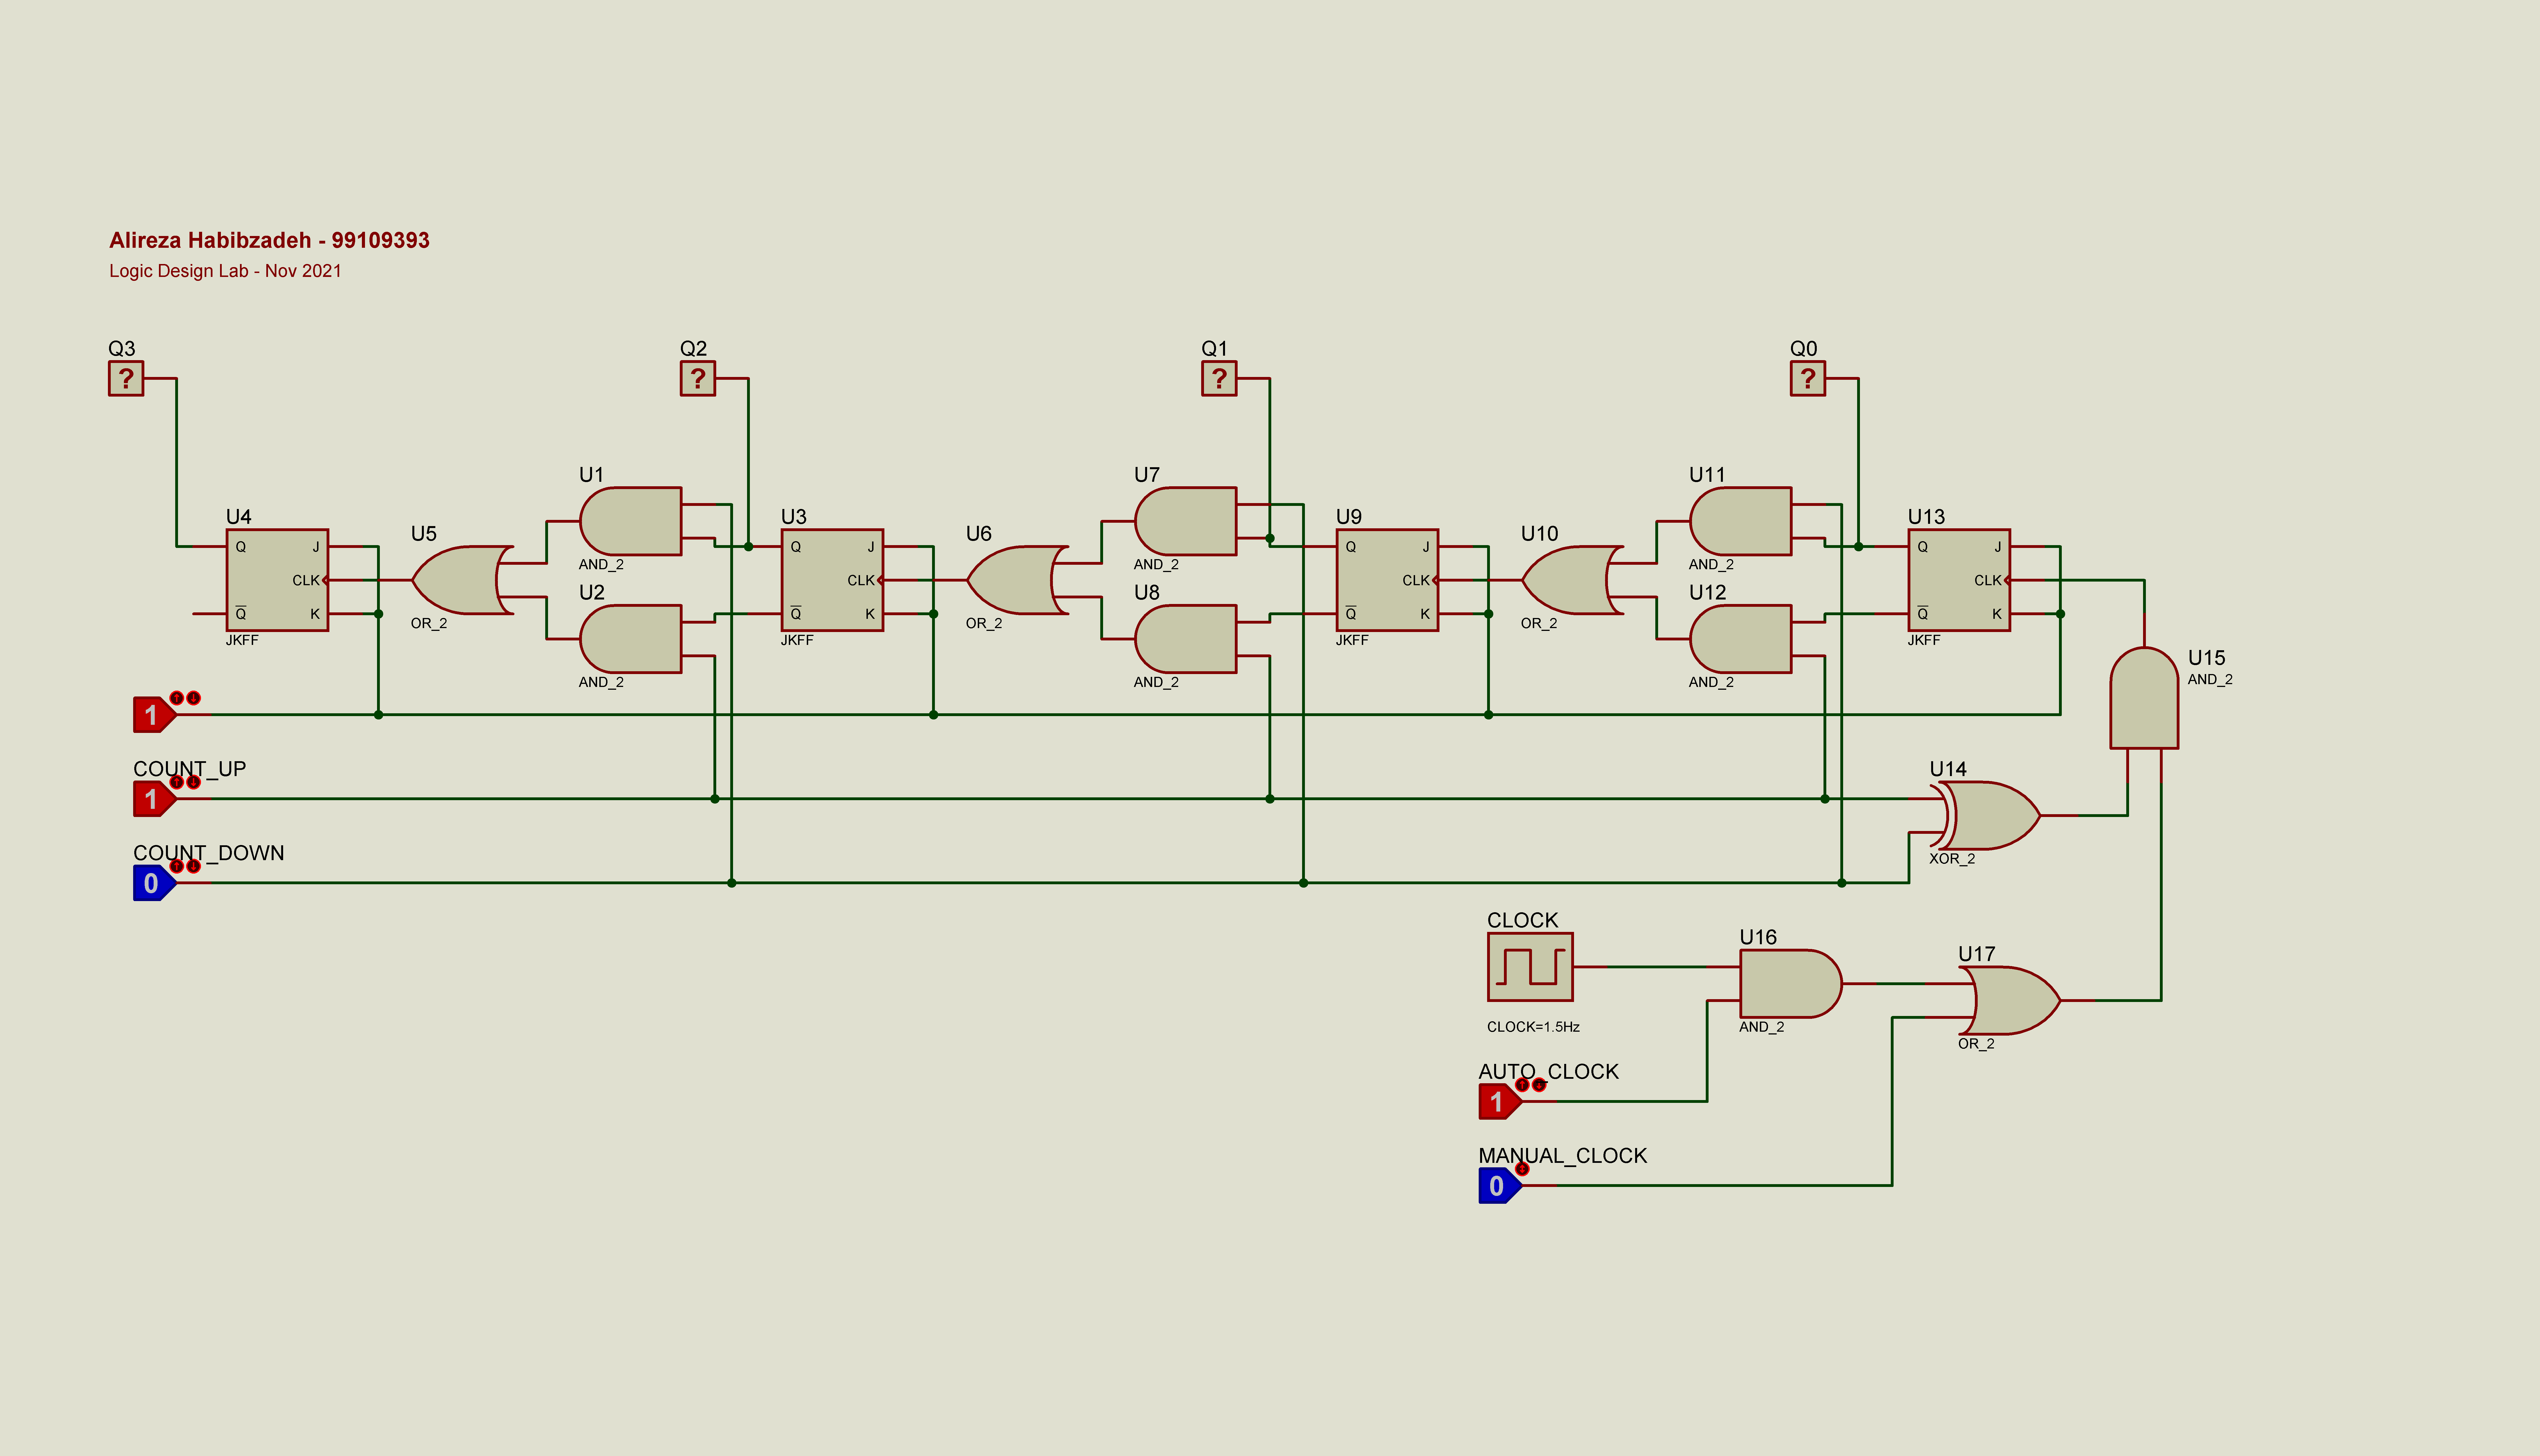
\includegraphics[width=\textwidth]{part1/1-1.png}
    \caption{
    شمارنده بالا
    /
    پایین شمار
    }
    \label{fig:circuit1}
\end{figure}



\section{
شمارنده بالا
/
پایین شمار
با قابلیت بارگذاری موازی
}
در این قسمت باید بارگذاری موازی را اضافه کنیم. برای این کار از ورودی‌های
set و
reset
فلیپ‌فلاپ‌ها استفاده می‌کنیم.
برای این کار در صورتی که می‌خواهیم یک خروجی ۱ شود
باید
set
را برابر با ۱ و reset را برابر
با ۰ قرار دهیم و برعکس.
برای انجام این کار
از دو گیت AND و
یک گیت NOT
برای هر خروجی استفاده شده است.

همچنین در برخی حالت‌ها نباید کلاک وارد مدار شود که کلاک ورودی با آن شرط
AND شده است.

در حالت آخر جدول ورودی هم نباید بارگذاری موازی کار کند پس ورودی
LOAD
با آن
AND
شده.

نتیجه‌ی نهایی در شکل
\eqref{fig:circuit2}
آمده است.

\begin{figure}
    \centering
    \includegraphics[width=\textwidth]{part1/1-2.png}
    \caption{
    شمارنده با قابلیت بارگذاری موازی
    }
    \label{fig:circuit2}
\end{figure}